
\subsection{Reveiwer Comments - \me{1}}

In this paper, the authors proposed a traffic aware resource allocation scheme for multi-cell MIMO-OFDM systems, where the precoders at all BSs are chosen to minimize the total user queue deviations. The problem is nonconvex and the authors proposed two centralized algorithms based on the successive approximation (SCA) technique to find a stationary point. Moreover, several distributed algorithms are also proposed using primal decomposition, alternating directions method of multipliers (ADMM), and decomposition via KKT conditions, respectively.

Most sections of this paper are well written. The results and algorithms also seem valid. However, the motivation of minimizing the total user queue deviations is not well justified. The convergence results of some algorithms are not clearly presented. The presentation of the distributed solutions needs significant improvement. Analysis and comparison of the signaling overhead and computational complexity between the centralized and distributed algorithms are also necessary to justify the advantages of distributed algorithms.

\resp We thank the reviewer for reading the paper and providing the comments. Please consider the responses in line with the comments.

\subsection*{Detailed Comments}  
\cmnt{1} In Section II.B, please provides more justifications for the problem formulation in (6). For example, the Queue weighted sum rate maximization (Q-WSRM) is throughput optimal, i.e., if there exists a scheme which can make all queues stable, then the Q-WSRM can also do this. How about the proposed formulation in (6)? Is it also throughput optimal? 

\resp We fully agree with the reviewer comment. The Q-WSRM scheme is throughput optimal when the queues associated with the users are significantly large in comparison with the transmission rate (service rate). In order to restrict the over allocation of the available resources to a specific user beyond the total number of queued packets, we have included the additional rate constraint in the Q-WSRME algorithm. It would be ideal to compare with the Q-WSRME algorithm which performs similar to the Q-WSRM when the queued packets are large enough to be emptied by the current transmissions. Fig. \ref{fig-review} compares the centralized algorithms using average number of backlogged packets after \me{100} slots of transmission for different arrival rate. Note that the average arrival rate of all the users are same but the instantaneous arrivals are based on the Poisson distribution. It can be seen from Fig. \ref{fig-review} that the JSFRA scheme with \me{q=2} performs similar to the Q-WSRME scheme for higher arrival rates, which explains the dropping of the squared rate term in the Q-WSRM formulation. When the average arrival rate is smaller, the JSFRA scheme with \me{q=2} performs noticeably better than the Q-WSRME scheme as can be seen from the average number of backlogged packets. In all packet arrival scenarios, JSFRA scheme with \me{q=1} reduces the average number of backlogged packets over the given slots is lesser than the Q-WSRME scheme.
\begin{figure}
\centering
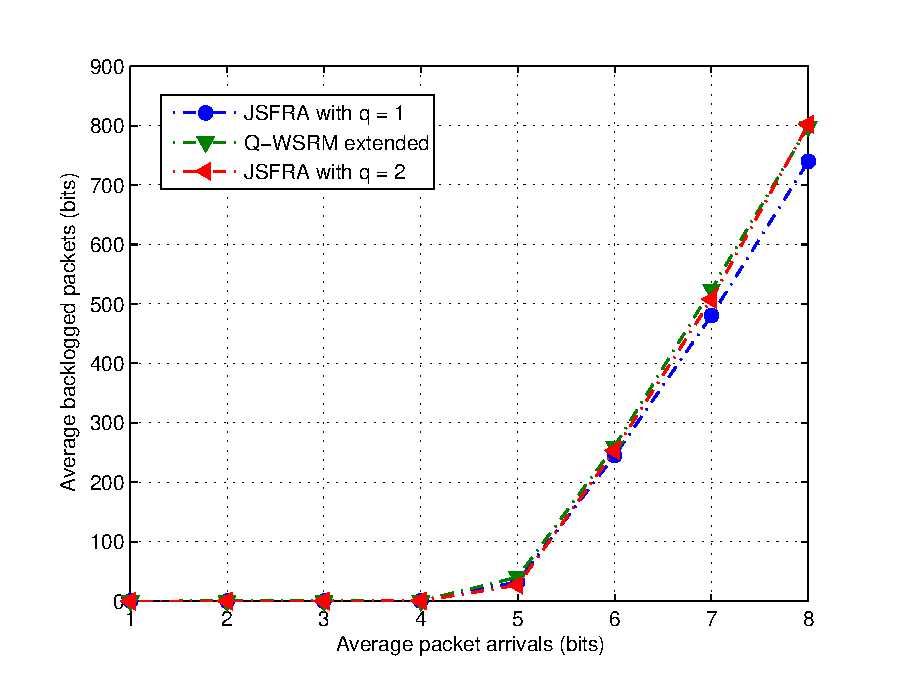
\includegraphics[width=\columnwidth]{Review/reviewer.eps}
\label{fig-review}
\caption{System \me{\lbrace N,N_B,K,N_R \rbrace = \lbrace 4,2,12,1 \rbrace}}
\end{figure}

\cmnt{2} Do the proposed solutions based on (6) achieve better average delay performance than the existing solutions? By the way, in the simulations, you should also add a figure comparing the average delay performance, instead of just comparing the performance metric defined by (6). This will better justify the advantage of the proposed solutions.

\resp We agree with the reviewer comment on the better average delay performance of Q-WSRM(E) approach over JSFRA scheme with \me{q=1} formulation. Note that the average delay can be reduced by including a convex minimum rate constraint in the JSFRA formulation to provide a guaranteed rate to all users or for certain users in the system. More over, the priority can also be incorporated easily in the formulation by the scaling factor \me{a_k} used in the formulation. As mentioned in Section \ref{sec-3.2}, the delay can also be addressed by using \me{q=2} or \me{q=\infty} norm objective in the JSFRA formulation.

\cmnt{3} In Section III.B, the convergence conditions under Algorithm 1 are not clear. First, you should be more specific about what is the SCA subproblem. Do you mean problem (19)? Second, does the uniqueness of the transmit and receive beamformers mean that the solution of the original problem in (16) is unique, or the solutions of the subproblems in (19) and (20) are unique, respectively?

\resp We understand the reviewer concerns. We have modified the convergence section to include additional information to provide more clarity. \review{Update converge proof}